\par
Recording frequency and activity during positive weeks provide a further decomposition of city-level intensity change. In the 36-city cohort, equal-city mean log-intensity change is \LongMeanI, combining +\LongMeanP{} from the frequency of positive records and +\LongMeanQ{} from positive-week activity minus \LongMeanN{} for facilities. Positive-record frequency does not decline in any city, and coded-zero weeks fall from \LongZeroStart{} to \LongZeroEnd{}; the long-window gap therefore occurs even as positive records become more prevalent.

The recent window separates the equal-city mean from the other summaries: its mean log-intensity change is positive (\RecentMeanI), while the median change and facility-weighted network intensity change are negative. The mean gives each city equal weight, whereas the facility-weighted ratio gives more influence to cities carrying more observed facilities. Low initial positive-week activity can also produce a large proportional increase, and a fall in positive-week frequency can accompany contraction despite complete calendar coverage. These components describe recorded-week structure; coded zeros remain observations under the source rule and are not treated as missing or as verified zero-transaction rates (Figure~\ref{fig:recording}). The full recording-frequency, positive-week and endpoint-support diagnostics are provided in SI Section~\siref{sec:si-descriptive}.
\begin{figure}[htbp]\centering
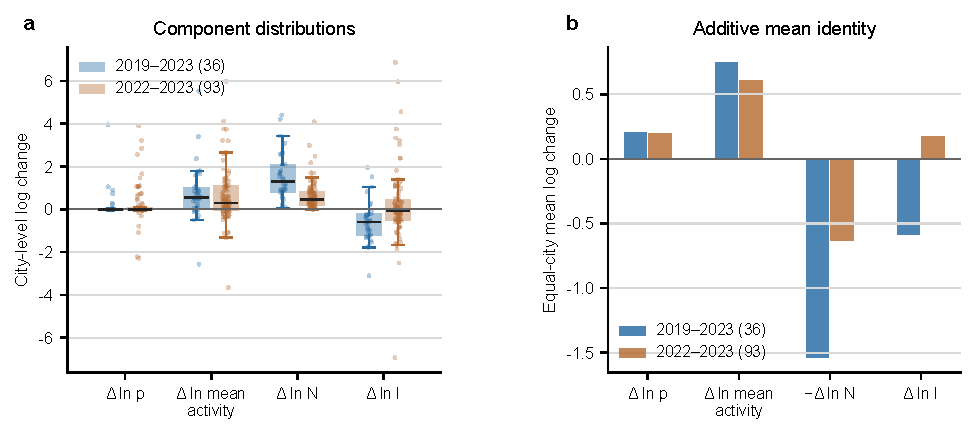
\includegraphics[width=\linewidth,height=.76\textheight,keepaspectratio]{figures/fig6_recording.pdf}
\caption{Recorded activity components and intensity changes}\label{fig:recording}
\end{figure}

